% Options for packages loaded elsewhere
\PassOptionsToPackage{unicode}{hyperref}
\PassOptionsToPackage{hyphens}{url}
%
\documentclass[
  man,floatsintext]{apa6}
\usepackage{amsmath,amssymb}
\usepackage{iftex}
\ifPDFTeX
  \usepackage[T1]{fontenc}
  \usepackage[utf8]{inputenc}
  \usepackage{textcomp} % provide euro and other symbols
\else % if luatex or xetex
  \usepackage{unicode-math} % this also loads fontspec
  \defaultfontfeatures{Scale=MatchLowercase}
  \defaultfontfeatures[\rmfamily]{Ligatures=TeX,Scale=1}
\fi
\usepackage{lmodern}
\ifPDFTeX\else
  % xetex/luatex font selection
\fi
% Use upquote if available, for straight quotes in verbatim environments
\IfFileExists{upquote.sty}{\usepackage{upquote}}{}
\IfFileExists{microtype.sty}{% use microtype if available
  \usepackage[]{microtype}
  \UseMicrotypeSet[protrusion]{basicmath} % disable protrusion for tt fonts
}{}
\makeatletter
\@ifundefined{KOMAClassName}{% if non-KOMA class
  \IfFileExists{parskip.sty}{%
    \usepackage{parskip}
  }{% else
    \setlength{\parindent}{0pt}
    \setlength{\parskip}{6pt plus 2pt minus 1pt}}
}{% if KOMA class
  \KOMAoptions{parskip=half}}
\makeatother
\usepackage{xcolor}
\usepackage{graphicx}
\makeatletter
\def\maxwidth{\ifdim\Gin@nat@width>\linewidth\linewidth\else\Gin@nat@width\fi}
\def\maxheight{\ifdim\Gin@nat@height>\textheight\textheight\else\Gin@nat@height\fi}
\makeatother
% Scale images if necessary, so that they will not overflow the page
% margins by default, and it is still possible to overwrite the defaults
% using explicit options in \includegraphics[width, height, ...]{}
\setkeys{Gin}{width=\maxwidth,height=\maxheight,keepaspectratio}
% Set default figure placement to htbp
\makeatletter
\def\fps@figure{htbp}
\makeatother
\setlength{\emergencystretch}{3em} % prevent overfull lines
\providecommand{\tightlist}{%
  \setlength{\itemsep}{0pt}\setlength{\parskip}{0pt}}
\setcounter{secnumdepth}{-\maxdimen} % remove section numbering
% Make \paragraph and \subparagraph free-standing
\ifx\paragraph\undefined\else
  \let\oldparagraph\paragraph
  \renewcommand{\paragraph}[1]{\oldparagraph{#1}\mbox{}}
\fi
\ifx\subparagraph\undefined\else
  \let\oldsubparagraph\subparagraph
  \renewcommand{\subparagraph}[1]{\oldsubparagraph{#1}\mbox{}}
\fi
\newlength{\cslhangindent}
\setlength{\cslhangindent}{1.5em}
\newlength{\csllabelwidth}
\setlength{\csllabelwidth}{3em}
\newlength{\cslentryspacingunit} % times entry-spacing
\setlength{\cslentryspacingunit}{\parskip}
\newenvironment{CSLReferences}[2] % #1 hanging-ident, #2 entry spacing
 {% don't indent paragraphs
  \setlength{\parindent}{0pt}
  % turn on hanging indent if param 1 is 1
  \ifodd #1
  \let\oldpar\par
  \def\par{\hangindent=\cslhangindent\oldpar}
  \fi
  % set entry spacing
  \setlength{\parskip}{#2\cslentryspacingunit}
 }%
 {}
\usepackage{calc}
\newcommand{\CSLBlock}[1]{#1\hfill\break}
\newcommand{\CSLLeftMargin}[1]{\parbox[t]{\csllabelwidth}{#1}}
\newcommand{\CSLRightInline}[1]{\parbox[t]{\linewidth - \csllabelwidth}{#1}\break}
\newcommand{\CSLIndent}[1]{\hspace{\cslhangindent}#1}
\ifLuaTeX
\usepackage[bidi=basic]{babel}
\else
\usepackage[bidi=default]{babel}
\fi
\babelprovide[main,import]{english}
% get rid of language-specific shorthands (see #6817):
\let\LanguageShortHands\languageshorthands
\def\languageshorthands#1{}
% Manuscript styling
\usepackage{upgreek}
\captionsetup{font=singlespacing,justification=justified}

% Table formatting
\usepackage{longtable}
\usepackage{lscape}
% \usepackage[counterclockwise]{rotating}   % Landscape page setup for large tables
\usepackage{multirow}		% Table styling
\usepackage{tabularx}		% Control Column width
\usepackage[flushleft]{threeparttable}	% Allows for three part tables with a specified notes section
\usepackage{threeparttablex}            % Lets threeparttable work with longtable

% Create new environments so endfloat can handle them
% \newenvironment{ltable}
%   {\begin{landscape}\centering\begin{threeparttable}}
%   {\end{threeparttable}\end{landscape}}
\newenvironment{lltable}{\begin{landscape}\centering\begin{ThreePartTable}}{\end{ThreePartTable}\end{landscape}}

% Enables adjusting longtable caption width to table width
% Solution found at http://golatex.de/longtable-mit-caption-so-breit-wie-die-tabelle-t15767.html
\makeatletter
\newcommand\LastLTentrywidth{1em}
\newlength\longtablewidth
\setlength{\longtablewidth}{1in}
\newcommand{\getlongtablewidth}{\begingroup \ifcsname LT@\roman{LT@tables}\endcsname \global\longtablewidth=0pt \renewcommand{\LT@entry}[2]{\global\advance\longtablewidth by ##2\relax\gdef\LastLTentrywidth{##2}}\@nameuse{LT@\roman{LT@tables}} \fi \endgroup}

% \setlength{\parindent}{0.5in}
% \setlength{\parskip}{0pt plus 0pt minus 0pt}

% Overwrite redefinition of paragraph and subparagraph by the default LaTeX template
% See https://github.com/crsh/papaja/issues/292
\makeatletter
\renewcommand{\paragraph}{\@startsection{paragraph}{4}{\parindent}%
  {0\baselineskip \@plus 0.2ex \@minus 0.2ex}%
  {-1em}%
  {\normalfont\normalsize\bfseries\itshape\typesectitle}}

\renewcommand{\subparagraph}[1]{\@startsection{subparagraph}{5}{1em}%
  {0\baselineskip \@plus 0.2ex \@minus 0.2ex}%
  {-\z@\relax}%
  {\normalfont\normalsize\itshape\hspace{\parindent}{#1}\textit{\addperi}}{\relax}}
\makeatother

\makeatletter
\usepackage{etoolbox}
\patchcmd{\maketitle}
  {\section{\normalfont\normalsize\abstractname}}
  {\section*{\normalfont\normalsize\abstractname}}
  {}{\typeout{Failed to patch abstract.}}
\patchcmd{\maketitle}
  {\section{\protect\normalfont{\@title}}}
  {\section*{\protect\normalfont{\@title}}}
  {}{\typeout{Failed to patch title.}}
\makeatother

\usepackage{xpatch}
\makeatletter
\xapptocmd\appendix
  {\xapptocmd\section
    {\addcontentsline{toc}{section}{\appendixname\ifoneappendix\else~\theappendix\fi\\: #1}}
    {}{\InnerPatchFailed}%
  }
{}{\PatchFailed}
\keywords{keywords\newline\indent Word count: X}
\usepackage{lineno}

\linenumbers
\usepackage{csquotes}
\ifLuaTeX
  \usepackage{selnolig}  % disable illegal ligatures
\fi
\IfFileExists{bookmark.sty}{\usepackage{bookmark}}{\usepackage{hyperref}}
\IfFileExists{xurl.sty}{\usepackage{xurl}}{} % add URL line breaks if available
\urlstyle{same}
\hypersetup{
  pdftitle={A cross-cultural universal of human social cognition: Children from 17 diverse communities process gaze in similar ways},
  pdfauthor={Manuel Bohn (ORCID: 0000-0001-6006-1348)1,2,*, Julia Prein (ORCID: 0000-0002-3154-6167)1,2,*, Agnes Ayikoru3, Florian M. Bednarski (ORCID: 0000-0003-4384-4791)4, Ardain Dzabatou5, Michael C. Frank (ORCID: 0000-0002-7551-4378)6, Annette M. E. Henderson (ORCID: 0000-0003-4384-4791)4, Joan Isabella3, Josefine Kalbitz2, Patricia Kanngiesser (ORCID:0000-0003-1068-3725)7, Dilara Keşşafoğlu (ORCID: 0000-0002-7356-0733)8, Bahar Köymen (ORCID: 0000-0001-5126-8240)9, Maira V. Manrique-Hernandez2, Shirley Magazi (ORCID: 0009-0006-0479-9800)10, Lizbeth Mújica-Manrique2, Julia Ohlendorf2, Damilola Olaoba2, Wesley R. Pieters (ORCID:0000-0002-6152-249X)10, Sarah Pope-Caldwell2, Katie Slocombe (ORCID: 0000-0002-7310-1887)11, Robert Z. Sparks (ORCID: 0000-0001-7545-0522)6, Jahnavi Sunderarajan2, Wilson Vieira2, Zhen Zhang (ORCID: 0000-0001-9300-0920)12, Yufei Zong (ORCID: 0009-0000-5012-0244)12, Roman Stengelin (ORCID: 0000-0003-2212-4613)2,10, \& Daniel B. M. Haun2},
  pdflang={en-EN},
  pdfkeywords={keywords},
  hidelinks,
  pdfcreator={LaTeX via pandoc}}

\title{A cross-cultural universal of human social cognition: Children from 17 diverse communities process gaze in similar ways}
\author{Manuel Bohn (ORCID: 0000-0001-6006-1348)\textsuperscript{1,2,*}, Julia Prein (ORCID: 0000-0002-3154-6167)\textsuperscript{1,2,*}, Agnes Ayikoru\textsuperscript{3}, Florian M. Bednarski (ORCID: 0000-0003-4384-4791)\textsuperscript{4}, Ardain Dzabatou\textsuperscript{5}, Michael C. Frank (ORCID: 0000-0002-7551-4378)\textsuperscript{6}, Annette M. E. Henderson (ORCID: 0000-0003-4384-4791)\textsuperscript{4}, Joan Isabella\textsuperscript{3}, Josefine Kalbitz\textsuperscript{2}, Patricia Kanngiesser (ORCID:0000-0003-1068-3725)\textsuperscript{7}, Dilara Keşşafoğlu (ORCID: 0000-0002-7356-0733)\textsuperscript{8}, Bahar Köymen (ORCID: 0000-0001-5126-8240)\textsuperscript{9}, Maira V. Manrique-Hernandez\textsuperscript{2}, Shirley Magazi (ORCID: 0009-0006-0479-9800)\textsuperscript{10}, Lizbeth Mújica-Manrique\textsuperscript{2}, Julia Ohlendorf\textsuperscript{2}, Damilola Olaoba\textsuperscript{2}, Wesley R. Pieters (ORCID:0000-0002-6152-249X)\textsuperscript{10}, Sarah Pope-Caldwell\textsuperscript{2}, Katie Slocombe (ORCID: 0000-0002-7310-1887)\textsuperscript{11}, Robert Z. Sparks (ORCID: 0000-0001-7545-0522)\textsuperscript{6}, Jahnavi Sunderarajan\textsuperscript{2}, Wilson Vieira\textsuperscript{2}, Zhen Zhang (ORCID: 0000-0001-9300-0920)\textsuperscript{12}, Yufei Zong (ORCID: 0009-0000-5012-0244)\textsuperscript{12}, Roman Stengelin (ORCID: 0000-0003-2212-4613)\textsuperscript{2,10}, \& Daniel B. M. Haun\textsuperscript{2}}
\date{}


\shorttitle{Gaze-following across 17 communities}

\authornote{

The authors would like to thank Luke Maurits for statistical advice. Manuel Bohn was supported by a Jacobs Foundation Research Fellowship (2022-1484-00). We are greatful to thank all children and caregivers for participating in the study.

The authors made the following contributions. Manuel Bohn (ORCID: 0000-0001-6006-1348): Conceptualization, Methodology, Formal Analysis, Writing - Original Draft Preparation, Writing - Review \& Editing; Julia Prein (ORCID: 0000-0002-3154-6167): Conceptualization, Methodology, Software, Investigation, Writing - Review \& Editing; Agnes Ayikoru: Investigation; Florian M. Bednarski (ORCID: 0000-0003-4384-4791): Investigation, Writing - Review \& Editing; Ardain Dzabatou: Investigation; Michael C. Frank (ORCID: 0000-0002-7551-4378): Investigation, Writing - Review \& Editing; Annette M. E. Henderson (ORCID: 0000-0003-4384-4791): Investigation, Writing - Review \& Editing; Joan Isabella: Investigation; Josefine Kalbitz: Investigation, Writing - Review \& Editing; Patricia Kanngiesser (ORCID:0000-0003-1068-3725): Investigation, Writing - Review \& Editing; Dilara Keşşafoğlu (ORCID: 0000-0002-7356-0733): Investigation, Writing - Review \& Editing; Bahar Köymen (ORCID: 0000-0001-5126-8240): Investigation, Writing - Review \& Editing; Maira V. Manrique-Hernandez: Investigation; Shirley Magazi (ORCID: 0009-0006-0479-9800): Investigation; Lizbeth Mújica-Manrique: Investigation, Writing - Review \& Editing; Julia Ohlendorf: Investigation; Damilola Olaoba: Investigation; Wesley R. Pieters (ORCID:0000-0002-6152-249X): Investigation, Writing - Review \& Editing; Sarah Pope-Caldwell: Investigation; Katie Slocombe (ORCID: 0000-0002-7310-1887): Investigation; Robert Z. Sparks (ORCID: 0000-0001-7545-0522): Investigation; Jahnavi Sunderarajan: Investigation; Wilson Vieira: Investigation; Zhen Zhang (ORCID: 0000-0001-9300-0920): Investigation, Writing - Review \& Editing; Yufei Zong (ORCID: 0009-0000-5012-0244): Investigation, Writing - Review \& Editing; Roman Stengelin (ORCID: 0000-0003-2212-4613): Conceptualization, Methodology, Investigation, Writing - Review \& Editing; Daniel B. M. Haun: Conceptualization, Funding acquisition, Writing - Review \& Editing.

Correspondence concerning this article should be addressed to Manuel Bohn (ORCID: 0000-0001-6006-1348), Universitätsallee 1, 21335 Lüneburg, Germany. E-mail: \href{mailto:manuel.bohn@leuphana.de}{\nolinkurl{manuel.bohn@leuphana.de}}

}

\affiliation{\vspace{0.5cm}\textsuperscript{1} Institute of Psychology in Education, Leuphana University Lüneburg\\\textsuperscript{2} Department of Comparative Cultural Psychology, Max Planck Institute for Evolutionary Anthropology\\\textsuperscript{3} Budongo Conservation Field Station\\\textsuperscript{4} School of Psychology, University of Auckland\\\textsuperscript{5} Université Marien Ngouabi\\\textsuperscript{6} Department of Psychology, Stanford University\\\textsuperscript{7} School of Psychology, University of Plymouth\\\textsuperscript{8} Department of Psychology, Koç University\\\textsuperscript{9} Division of Psychology, Communication, and Human Neuroscience, University of Manchester\\\textsuperscript{10} Department of Psychology and Social Work, University of Namibia\\\textsuperscript{11} Department of Psychology, University of York\\\textsuperscript{12} CAS Key Laboratory of Behavioral Science, Institute of Psychology, Chinese Academy of Sciences\\\textsuperscript{*} joint first author}

\abstract{%
Theoretical accounts assume that key features of human social cognition are universal. Here we focus on gaze following, the bedrock of social interactions and coordinated activities, to test this claim. In this comprehensive cross-cultural study spanning five continents and 17 distinct cultural communities, we examined the development of gaze following in early childhood. We identified key processing signatures through a computational model that assumes that participants follow an individual's gaze by estimating a vector emanating from the eye-center through the pupil. Using a single reliable touchscreen-based task, we found these signatures in all communities, suggesting that children worldwide processed gaze in highly similar ways. Additionally, we found a cross-culturally consistent relationship between children's exposure to touchscreens and their performance in the task, which also explained absolute differences between communities. These results provide strong evidence for a universal process underlying a foundational socio-cognitive ability in humans that can be reliably inferred even in the presence of cultural variation in overt behavior.
}



\begin{document}
\maketitle

Human socio-cognitive skills enable unique forms of communication and cooperation that provide a bedrock for cumulative culture and the formation of complex societies (\emph{1}--\emph{7}). The eyes are the proverbial ``window to the mind'' and eye gaze is essential for many social reasoning processes (\emph{8}, \emph{9}). Others' eye gaze is used to infer their focus of visual attention, which is a critical aspect of coordinated activities, including communication and cooperation (\emph{10}, \emph{11}). The ability to follow gaze emerges early in childhood (\emph{12}--\emph{15}) and individual differences in children's gaze-following ability predict later life outcomes, most notably, communicative abilities (\emph{16}, \emph{17}). Difficulties with gaze following have been linked to developmental disorders, including Autism (\emph{18}).

There is a widely-held assumption, that, despite substantial variation in developmental contexts, gaze-following works and develops in the same way across human societies (\emph{19}). However, this view is seemingly at odds with the substantial diversity in socio-cognitive development that cross-cultural studies have revealed (\emph{3}, \emph{20}--\emph{23}). One potential source for this paradox lies in the reliance on aggregated measures in cross-cultural studies. Absolute differences in mean performance across communities are interpreted as a signal of different underlying cognitive processes. In this study, we resolve this paradox by instead focusing on processing signatures that can be investigated independently of absolute community-level differences. This allows us to directly evaluate the empirical foundation of claims about universal features of human social cognition. To this end, we conducted a pre-registered, large-scale, cross-cultural study on the development of gaze-following abilities to study potentially universal processing signatures. These signatures were derived from a computational model that assumes that participants follow gaze by estimating a vector emanating from the eye center through the pupil (\emph{24}).

The 1377 participants who took part in the study lived in 17 different communities across 14 countries and five continents (Fig. \ref{fig:fig1}A, Tab. \ref{tab:tab1}). These countries represent \textasciitilde46\% of the world's population. Communities covered a broad spectrum of geographical locations, social and political systems, languages, and subsistence styles (see Supplemental Materials). This diversity allowed us to overcome the common pitfall of cross-cultural studies that largely compared urban communities from the global north to rural communities from the global south (\emph{25}).

\begin{figure}

{\centering 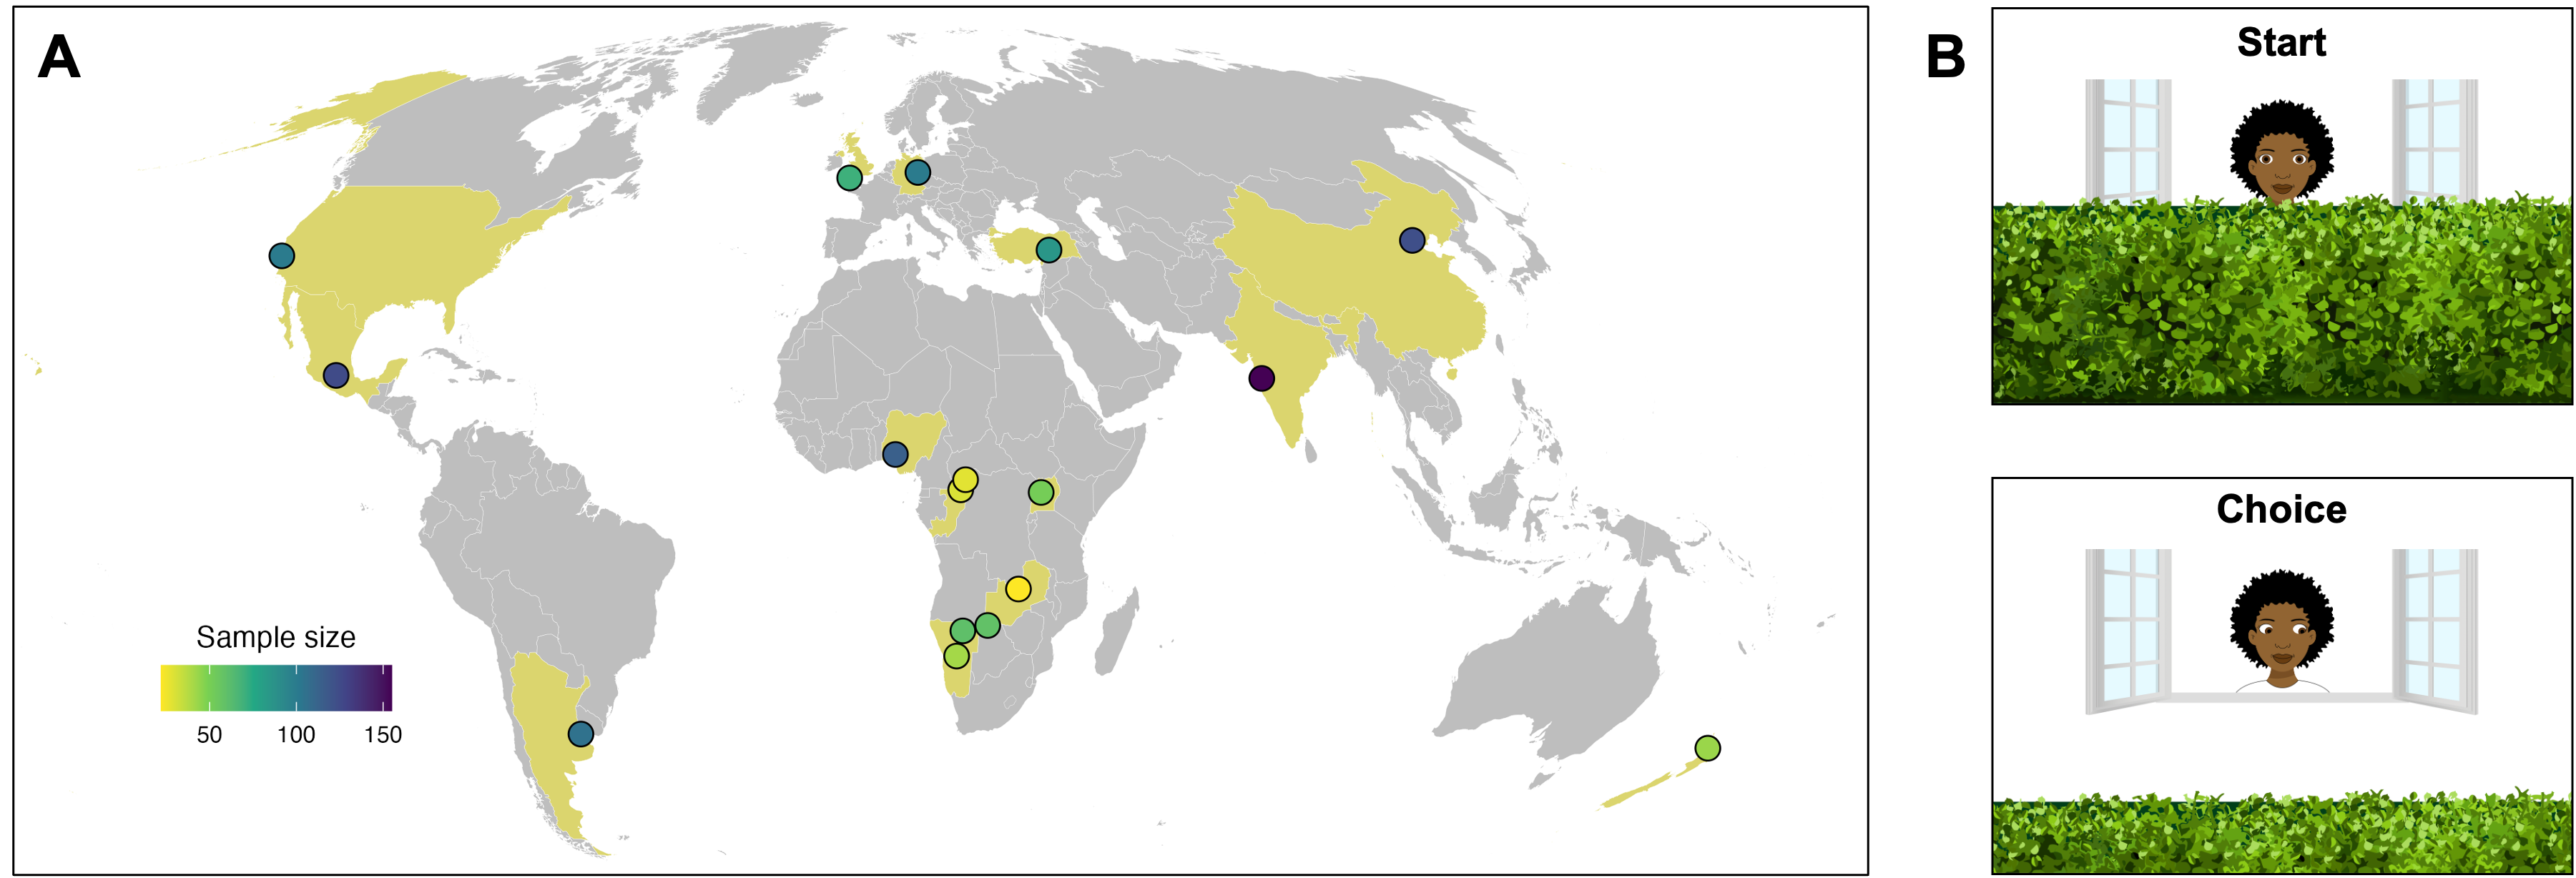
\includegraphics[width=0.75\linewidth]{../visuals/fig1} 

}

\caption{(A) Data collection sites. Points show the approximate geographical location of the data collection sites, coloring shows the sample sizes. (B) Screenshot from the task. The scene depicts the choice phase in a test trial. Participants had to use the gaze of the agent to locate the balloon and click on the location on the hedge where they thought the balloon was. Agents, audio recordings and backgrounds were adapted to each cultural setting. (C) Drawings used as agents across cultural settings. (D) Graphical illustration of the cognitive model. Individuals infer the target of an agent’s attention by estimating a vector based on the position of the pupils within the eyes. This process is noisy, illustrated by the different vectors (transparent lines). Individuals differ in their level of precision (indicated by sigma). For a given level of precision, the closer the  target lands to the left or the right, the less precise the model predicts individuals to be. Solid and transparent dots show simulated means and individual data points to illustrate the predicted effect of target position.}\label{fig:fig1}
\end{figure}

\begin{center}
\begin{ThreePartTable}

\begin{TableNotes}[para]
\normalsize{\textit{Note.} *Local collaborators and piloting suggested that Nigerian English is suitable for Windhoek as well.}
\end{TableNotes}

\begin{longtable}{m{0.111111111111111\linewidth}m{0.111111111111111\linewidth}m{0.111111111111111\linewidth}m{0.111111111111111\linewidth}m{0.111111111111111\linewidth}m{0.111111111111111\linewidth}m{0.111111111111111\linewidth}m{0.111111111111111\linewidth}}\noalign{\getlongtablewidth\global\LTcapwidth=\longtablewidth}
\caption{\label{tab:tab1}Participant demographics.}\\
\toprule
Continent & Country & Community & N(male) & Age (range) & Language & Market integration & Touchscreen\\
\midrule
\endfirsthead
\caption*{\normalfont{Table \ref{tab:tab1} continued}}\\
\toprule
Continent & Country & Community & N(male) & Age (range) & Language & Market integration & Touchscreen\\
\midrule
\endhead
Americas & Argentina & Buenos Aires & 105 (53) & 4.72 (3.00 - 6.96) & Spanish (Rioplatense) & high & 0.90\\
 & México & Ocuilan & 127 (63) & 4.96 (2.57 - 6.95) & Spanish (Mexican) & medium & 0.77\\
 & USA & Stanford & 98 (54) & 4.99 (2.52 - 7.90) & English (American) & high & 0.98\\
Africa & Namibia & Hai||om & 60 (38) & 5.85 (2.74 - 8.34) & Hai||om & low & 0.05\\
 &  & Khwe & 59 (24) & 5.84 (3.38 - 8.63) & Khwedam & low & 0.19\\
 &  & Windhoek & 39 (17) & 5.69 (2.66 - 8.66) & English (Nigerian) & high & 0.95\\
 & Nigeria & Akure & 114 (54) & 5.07 (2.57 - 7.33) & English (Nigerian)* & high & 0.91\\
 & Rep. Congo & BaYaka & 29 (13) & 7.80 (3.94 - 10.56) & BaYaka & low & 0.00\\
 &  & Bandongo & 30 (11) & 7.45 (3.50 - 10.95) & Lingala & low & 0.00\\
 & Uganda & Nyabyeya & 125 (62) & 5.94 (2.67 - 8.92) & Swahili & medium & 0.34\\
 & Zambia & Chimfunshi & 22 (5) & 5.98 (2.88 - 8.00) & Bemba & medium & 0.14\\
Europe & Germany & Leipzig & 100 (48) & 4.88 (2.53 - 6.95) & German & high & 0.89\\
 & UK & Plymouth & 70 (30) & 6.02 (2.38 - 8.94) & English (British) & high & 0.99\\
Asia & China & Beijing & 123 (62) & 5.47 (2.69 - 8.48) & Mandarin & high & 0.95\\
 & India & Pune & 148 (73) & 6.14 (3.06 - 8.83) & English (Indian) / Marathi & high & 0.93\\
 & Türkiye & Malatya & 85 (40) & 5.02 (2.75 - 7.12) & Turkish & high & 1.00\\
Oceania & New Zealand & Auckland & 43 (19) & 5.14 (2.81 - 8.75) & English (New Zealand) & high & 0.95\\
\bottomrule
\addlinespace
\insertTableNotes
\end{longtable}

\end{ThreePartTable}
\end{center}

We used an animated picture book tablet task in which participants had to locate a hidden object based on observing an agent's gaze. Children watched a balloon disappear behind a hedge. An agent followed the trajectory of the balloon with their eyes (Fig. \ref{fig:fig1}B). The key dependent variable was the (im)precision with which children located the agent's focus of attention, that is, the deviation between where the agent looked (where the object was) and the child's response. We adapted visuals and audio instructions specifically to each of the 17 communities. Previous work demonstrated excellent individual-level measurement properties for this task in a German sample (\emph{26}).

As the first step, we investigated developmental improvements, that is, how children become more precise at estimating the target location with age. Across all 17 communities, we found a substantial increase in average levels of precision with age (fixed effect in Bayesian regression model (\emph{27}): \(\beta\) = -0.30, 95\% HDI (-0.40 - -0.21); range of community-level (random) effects: \(\beta_{min}\) = -0.06, 95\% HDI (-0.18 - 0.05) to \(\beta_{max}\) = -0.59, 95\% HDI (-0.71 - -0.48).

Nevertheless, there were also marked differences between communities (see Fig. \ref{fig:fig2}A). In a six-fold cross-validation procedure, we trained a regression model on a subset of the data (training data) to later predict the held-out data (testing data) (\emph{28}). We found that a model assuming cross-cultural variation in average performance as well as cross-cultural variation in developmental trajectories outperformed simpler models -- assuming no variation in the shape of developmental trajectories or nor variation between settings at all -- in 98\% of cases (see Supplemental Material). At first glance, it seems that highly market-integrated communities around the globe showed higher levels of precision compared to less market-integrated communities (compare Tab. \ref{tab:tab1} and Fig. \ref{fig:fig2}A). However, numerous alternative groupings (e.g., average levels of education or average household size) are possible and, instead, these results could be best understood in terms of exposure to touch-screen devices; a finding we discuss in more detail below. Importantly, average differences in precision between communities were small compared to differences between individuals: communities did not form homogeneous clusters but largely overlapping distributions in that some individuals from communities with a lower average level of precision performed better compared to some individuals from a setting with a very high average level of precision. Similarly, in all communities, some 4-year-olds outperformed children two years older than them (see Fig. \ref{fig:fig2}A). The lack of adequate individual-level measurement instruments in previous large-scale developmental cross-cultural studies made it impossible to contrast these perspectives. The substantial overlap between communities found here speaks against categorical differences in gaze following and is suggestive of a similar underlying process. However, consistent developmental improvements alone cannot inform us about the cognitive processes children use when locating the agent's focus of attention.

\begin{figure}

{\centering 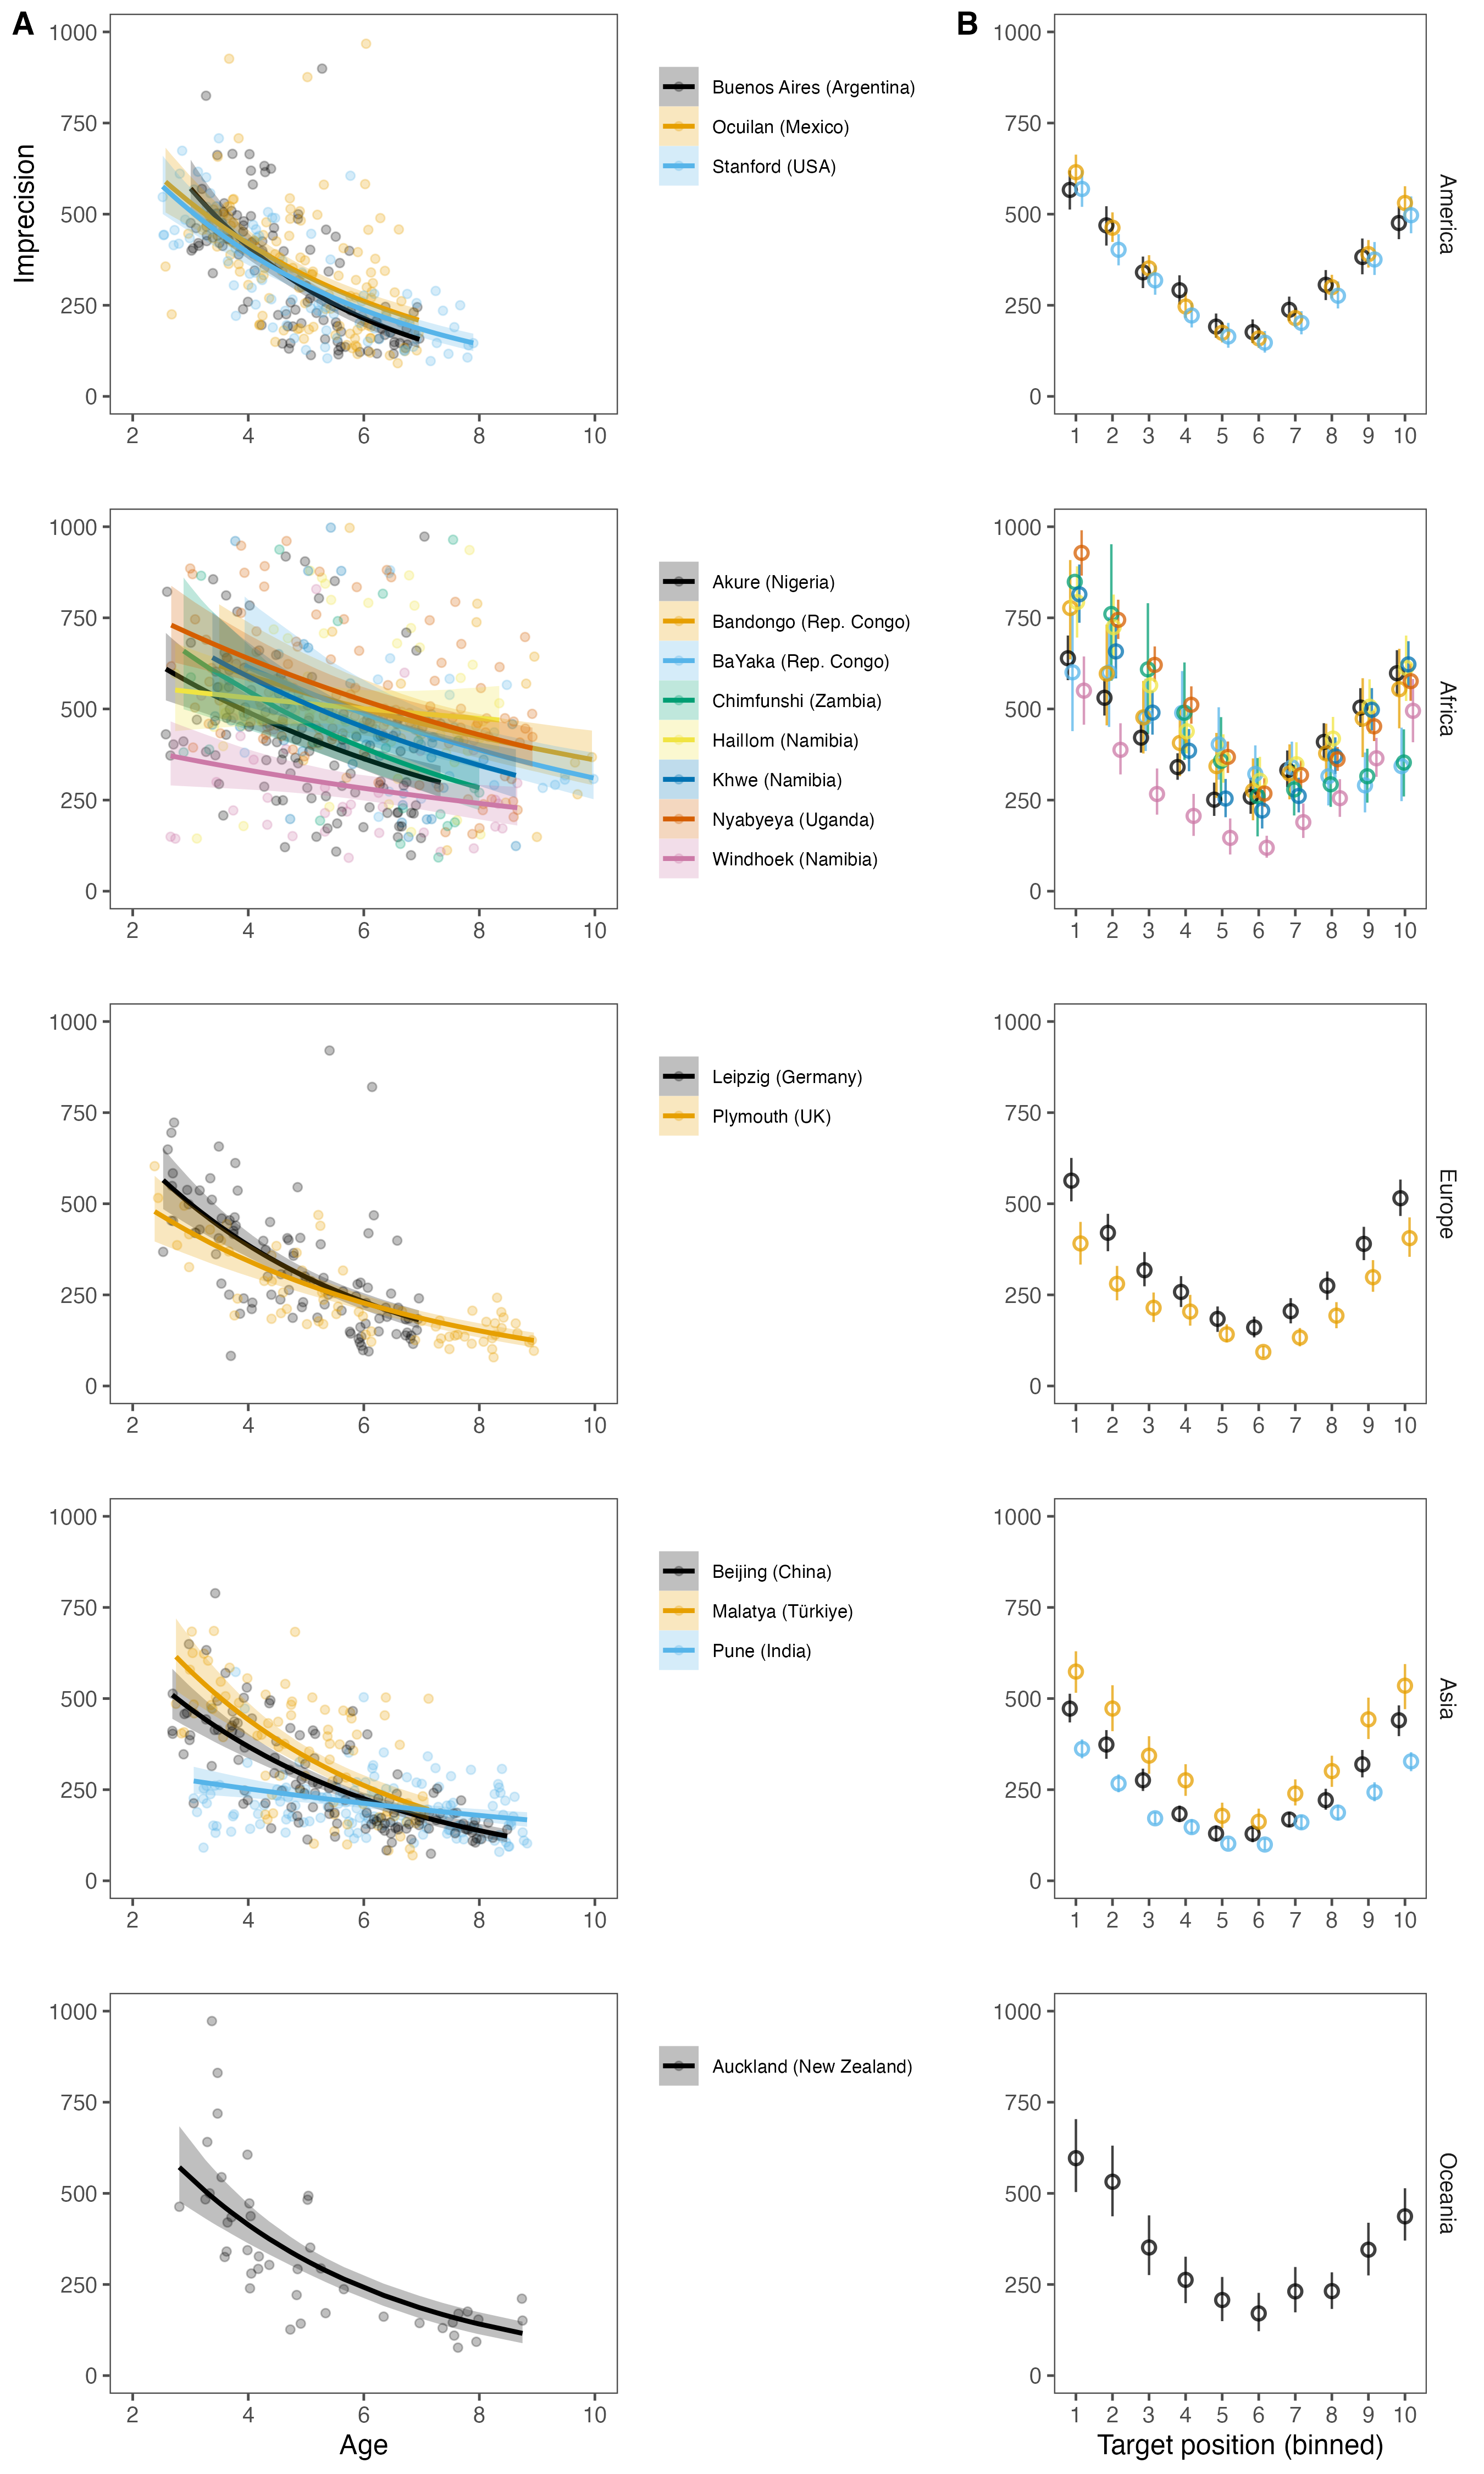
\includegraphics[width=1\linewidth]{../visuals/pvis_pred} 

}

\caption{A) Developmental trajectory across and B) by community. The developmental trajectories are predicted based on a model of the data aggregated for each participant. C) Performance by screen section across and D) by community. Each bin covers 1/10th of the screen. Points show means, and error bars 95\% confidence intervals for the data within that bin aggregated across participants. Transparent dots in A) and C) show aggregated data for each individual.}\label{fig:fig2}
\end{figure}

Recent computational work modeled gaze following as social vector estimation (\emph{24}). When observing the eyes, onlookers estimate a vector emanating from the center of the eye that runs through the pupil. The focus of attention is the location where the estimated vectors from both eyes hit a surface (Fig. \ref{fig:fig1}D). It is assumed that this estimation process has some uncertainty and that individuals vary in their level of uncertainty. As a consequence, even though individuals use the same general process, they might differ in their absolute levels of precision. Crucially, this process model predicts a clear performance signature in our gaze following task: Trials in which the agent looks further away from the center (i.e.~to the left or right side of the screen) should result in lower levels of precision compared to trials in which the agent looks closer to the middle. This prediction is best understood by considering a similar phenomenon: pointing a torch light to a flat surface. The width of the light beam represents each individual's level of uncertainty in vector estimation. When the torch is directed straight down, the light beam is concentrated in a relatively small area. When the torch is rotated to the side, the light from one half of the cone must travel further than the light from the other half to reach the surface. As a consequence, the light is spread over a wider area (see Fig. \ref{fig:fig1}D).

This processing signature was clearly visible across all 17 communities. Precision decreased when the agent looked at locations further away from the center (fixed effect: \(\beta\) = 0.47, 95\% HDI ( - 0.54); range of community-level effects: \(\beta_{min}\) = 0.58, 95\% HDI (0.51 - 0.66) to \(\beta_{max}\) = 0.16, 95\% HDI (-0.01 - 0.33). Visualization of the data showed the predicted u-shaped pattern in all communities (see Fig. \ref{fig:fig2}B). These results indicate a universal cognitive process used by children in all communities. There are, however, alternative ways in which the u-shaped pattern might arise: if participants ignored the agent's gaze and instead always selected the middle of the screen (center bias) or randomly select locations (random guessing), precision would also decrease when the balloon lands further away from the center. To rule out these alternative explanations, we compared three cognitive models that made different assumptions about how participants' responses were generated: the focal vector-based gaze estimation model described above, a center-bias model where participants always select the center, and a random guessing model where participants select random locations. For every community, we found overwhelming support for the gaze estimation model (min \(BF_{10}\) \textgreater{} 100 000 for comparisons with both alternative models). Taken together, children from all 17 communities processed gaze in similar ways.

Next, we looked at factors that could explain community- and individual-level variation. In addition to the gaze-following task, caregivers responded to a short questionnaire about children's access to screen-based technology and household composition. On an individual level, we found that children with access to touchscreen devices had higher levels of precision (\(\beta\) = -0.14, SE = 0.04, 95\% CrI = -0.21 - -0.07). This effect was consistent across communities in that allowing the effect of access to touchscreens to vary across communities did not improve model fit (see Supplemental Materials). On a community level, we also saw that average performance was lowest in communities in which touchscreen devices were the least frequent (community-level correlation between age-corrected imprecision and proportion of children with access to touchscreens: \emph{r} = -0.90, 95\% CI = -0.96 - -0.74). Thus, familiarity with the device used for data collection likely explains variation between communities. The most likely explanation for this effect is that children with more touchscreen experience were better at task handling and thus more likely to precisely touch the location they inferred the agent to look at.

However, there was substantial variation between individuals that could not be explained by differential exposures to touch screens alone. For example, in Malatya (Türkyie) where 100\% of children had access to touch screens there was still substantial variation between individuals (see Fig. 1B). This strongly indicates that other factors likely contributed to individual differences. Social interaction has been highlighted as an important driver of social-cognitive development (e.g., \emph{19}, \emph{29}--\emph{32}) and thus we hypothesized (and pre-registered) that more opportunities for social interaction -- approximated by living in larger households with more children -- would be associated with higher levels of precision. At first glance, the opposite seemed to be the case: there was a substantial zero-order correlation between the number of children living in the household and average imprecision (0.27, 95\% CI = 0.22 - 0.32) suggesting that having more opportunities for social interactions was related to poorer performance. However, this correlation is spurious and reflects a confounding of household composition with exposure to technology on a community level. When predicting performance by relative opportunities for social interactions within a community -- while accounting for absolute differences and the prevalence of touchscreens -- we found no strong associations between any of the demographic indicators and performance (see Supplemental Material). The reason for an absence of such an association may be a lack of resolution: household composition is very far removed from the factors that previous work has suggested to be related to the development of gaze following in younger children, such as attachment quality or the use of gaze in early communicative interactions (\emph{33}--\emph{35}). Future work could increase the resolution with which everyday experiences in children from diverse communities are recorded to compare the drivers behind development as we observe it. Recent work in the field of language acquisition has shown how technological innovations allowed for direct recording of social interactions across communities which can be used to close this explanatory gap (\emph{36}, \emph{37}).

Following and understanding gaze is a foundational building block of human social cognition (\emph{10}, \emph{11}). A substantial body of work has explored the developmental onset of gaze following in a few selected cultural communities (\emph{12}--\emph{14}, \emph{38}). The data reported here provides strong evidence that children from a large and diverse set of communities process others' gaze in similar ways. We found key performance signatures of a model treating gaze following as a form of social vector estimation across all 17 communities. With the focus on individual-level processing signatures, the study goes beyond previous studies on gaze following -- focused on the onset of gaze following in infancy (\emph{39}, \emph{40}) -- as well as comprehensive cross-cultural studies that compared average developmental trajectories (\emph{41}--\emph{44}).

The cognitive processes underlying gaze following might be rooted in humans' evolved cognitive architecture, which is -- presumably -- later refined during social (i.e., cultural) interaction (\emph{33}--\emph{35}). The phylogenetic roots of these processes might possibly lie much deeper as primates from a wide range of species follow gaze (\emph{45}--\emph{48}). Yet, similarities in overt behavior do not imply the same underlying cognitive processes. The present study defines clear performance signatures that can be explored in other species to test such evolutionary hypotheses.

Our study combined precise individual-level cognitive measurement and individual-level assessment of experience (here: touchscreen exposure) in a large and diverse sample to directly investigate the impact of specific cultural experiences on developmental outcomes. Instead of establishing universality by maximizing the cultural distance between two or three tested communities (\emph{49}), this large-scale cross-cultural approach treats children's cultural experience at scale, shedding light on the big ``middle ground'' of children's cultural experience (\emph{25}).

In sum, our work pioneers an approach that introduces computational modeling and precise individual-level measurement to the cross-cultural study of cognitive development. This approach allowed us to test for universals in the human cognitive architecture rather than just overt behavior. As such, it can serve as a blueprint for future research on a broad spectrum of cognitive abilities and offers a much-needed empirical foundation for theories on the nature of the human mind. Children from diverse cultures deploy similar cognitive processes in interpreting gaze, pointing to a universal foundation of basic social cognition, which is refined during development.

\newpage

\hypertarget{references}{%
\section{References}\label{references}}

\hypertarget{refs}{}
\begin{CSLReferences}{0}{0}
\leavevmode\vadjust pre{\hypertarget{ref-tomasello2020adaptive}{}}%
\CSLLeftMargin{1. }%
\CSLRightInline{M. Tomasello, The adaptive origins of uniquely human sociality. \emph{Philosophical Transactions of the Royal Society B} \textbf{375}, 20190493 (2020).}

\leavevmode\vadjust pre{\hypertarget{ref-laland2021understanding}{}}%
\CSLLeftMargin{2. }%
\CSLRightInline{K. Laland, A. Seed, Understanding human cognitive uniqueness. \emph{Annual Review of Psychology} \textbf{72}, 689--716 (2021).}

\leavevmode\vadjust pre{\hypertarget{ref-wellman2014making}{}}%
\CSLLeftMargin{3. }%
\CSLRightInline{H. M. Wellman, \emph{Making Minds: How Theory of Mind Develops} (Oxford University Press, 2014).}

\leavevmode\vadjust pre{\hypertarget{ref-henrich2016secret}{}}%
\CSLLeftMargin{4. }%
\CSLRightInline{J. Henrich, \emph{The Secret of Our Success: How Culture Is Driving Human Evolution, Domesticating Our Species, and Making Us Smarter} (princeton University press, 2016).}

\leavevmode\vadjust pre{\hypertarget{ref-tomasello2003makes}{}}%
\CSLLeftMargin{5. }%
\CSLRightInline{M. Tomasello, H. Rakoczy, What makes human cognition unique? From individual to shared to collective intentionality. \emph{Mind \& language} \textbf{18}, 121--147 (2003).}

\leavevmode\vadjust pre{\hypertarget{ref-legare2019development}{}}%
\CSLLeftMargin{6. }%
\CSLRightInline{C. H. Legare, The development of cumulative cultural learning. \emph{Annual Review of Developmental Psychology} \textbf{1}, 119--147 (2019).}

\leavevmode\vadjust pre{\hypertarget{ref-heyes2018cognitive}{}}%
\CSLLeftMargin{7. }%
\CSLRightInline{C. Heyes, \emph{Cognitive Gadgets} (Harvard University Press, 2018).}

\leavevmode\vadjust pre{\hypertarget{ref-shepherd2010following}{}}%
\CSLLeftMargin{8. }%
\CSLRightInline{S. V. Shepherd, Following gaze: Gaze-following behavior as a window into social cognition. \emph{Frontiers in integrative neuroscience} \textbf{4}, 5 (2010).}

\leavevmode\vadjust pre{\hypertarget{ref-doherty2006development}{}}%
\CSLLeftMargin{9. }%
\CSLRightInline{M. J. Doherty, The development of mentalistic gaze understanding. \emph{Infant and Child Development} \textbf{15}, 179--186 (2006).}

\leavevmode\vadjust pre{\hypertarget{ref-tomasello2007reliance}{}}%
\CSLLeftMargin{10. }%
\CSLRightInline{M. Tomasello, B. Hare, H. Lehmann, J. Call, Reliance on head versus eyes in the gaze following of great apes and human infants: The cooperative eye hypothesis. \emph{Journal of Human Evolution} \textbf{52}, 314--320 (2007).}

\leavevmode\vadjust pre{\hypertarget{ref-scaife1975capacity}{}}%
\CSLLeftMargin{11. }%
\CSLRightInline{M. Scaife, J. S. Bruner, The capacity for joint visual attention in the infant. \emph{Nature} \textbf{253}, 265--266 (1975).}

\leavevmode\vadjust pre{\hypertarget{ref-tang2023slow}{}}%
\CSLLeftMargin{12. }%
\CSLRightInline{Y. Tang, M. R. Gonzalez, G. O. Deák, The slow emergence of gaze-and point-following: A longitudinal study of infants from 4 to 12 months. \emph{Developmental Science}, e13457 (2023).}

\leavevmode\vadjust pre{\hypertarget{ref-gredeback2010development}{}}%
\CSLLeftMargin{13. }%
\CSLRightInline{G. Gredebäck, L. Fikke, A. Melinder, The development of joint visual attention: A longitudinal study of gaze following during interactions with mothers and strangers. \emph{Developmental science} \textbf{13}, 839--848 (2010).}

\leavevmode\vadjust pre{\hypertarget{ref-byers2021development}{}}%
\CSLLeftMargin{14. }%
\CSLRightInline{K. Byers-Heinlein, R. K.-Y. Tsui, D. Van Renswoude, A. K. Black, R. Barr, A. Brown, M. Colomer, S. Durrant, A. Gampe, N. Gonzalez-Gomez, others, The development of gaze following in monolingual and bilingual infants: A multi-laboratory study. \emph{Infancy} \textbf{26}, 4--38 (2021).}

\leavevmode\vadjust pre{\hypertarget{ref-del2019developmental}{}}%
\CSLLeftMargin{15. }%
\CSLRightInline{T. Del Bianco, T. Falck-Ytter, E. Thorup, G. Gredebäck, The developmental origins of gaze-following in human infants. \emph{Infancy} \textbf{24}, 433--454 (2019).}

\leavevmode\vadjust pre{\hypertarget{ref-brooks2005development}{}}%
\CSLLeftMargin{16. }%
\CSLRightInline{R. Brooks, A. N. Meltzoff, The development of gaze following and its relation to language. \emph{Developmental science} \textbf{8}, 535--543 (2005).}

\leavevmode\vadjust pre{\hypertarget{ref-carpenter1998social}{}}%
\CSLLeftMargin{17. }%
\CSLRightInline{M. Carpenter, K. Nagell, M. Tomasello, G. Butterworth, C. Moore, Social cognition, joint attention, and communicative competence from 9 to 15 months of age. \emph{Monographs of the society for research in child development}, i--174 (1998).}

\leavevmode\vadjust pre{\hypertarget{ref-itier2009neural}{}}%
\CSLLeftMargin{18. }%
\CSLRightInline{R. J. Itier, M. Batty, Neural bases of eye and gaze processing: The core of social cognition. \emph{Neuroscience \& Biobehavioral Reviews} \textbf{33}, 843--863 (2009).}

\leavevmode\vadjust pre{\hypertarget{ref-tomasello2019becoming}{}}%
\CSLLeftMargin{19. }%
\CSLRightInline{M. Tomasello, \emph{Becoming Human: A Theory of Ontogeny} (Harvard University Press, 2019).}

\leavevmode\vadjust pre{\hypertarget{ref-miller2018contributions}{}}%
\CSLLeftMargin{20. }%
\CSLRightInline{J. G. Miller, M. Wice, N. Goyal, Contributions and challenges of cultural research on the development of social cognition. \emph{Developmental Review} \textbf{50}, 65--76 (2018).}

\leavevmode\vadjust pre{\hypertarget{ref-mayer2013synchrony}{}}%
\CSLLeftMargin{21. }%
\CSLRightInline{A. Mayer, B. E. Träuble, Synchrony in the onset of mental state understanding across cultures? A study among children in samoa. \emph{International Journal of Behavioral Development} \textbf{37}, 21--28 (2013).}

\leavevmode\vadjust pre{\hypertarget{ref-dixson2018scaling}{}}%
\CSLLeftMargin{22. }%
\CSLRightInline{H. G. Dixson, A. F. Komugabe-Dixson, B. J. Dixson, J. Low, Scaling theory of mind in a small-scale society: A case study from vanuatu. \emph{Child Development} \textbf{89}, 2157--2175 (2018).}

\leavevmode\vadjust pre{\hypertarget{ref-taumoepeau2019cross}{}}%
\CSLLeftMargin{23. }%
\CSLRightInline{M. Taumoepeau, S. Sadeghi, A. Nobilo, Cross-cultural differences in children's theory of mind in iran and new zealand: The role of caregiver mental state talk. \emph{Cognitive Development} \textbf{51}, 32--45 (2019).}

\leavevmode\vadjust pre{\hypertarget{ref-prein2023variation}{}}%
\CSLLeftMargin{24. }%
\CSLRightInline{J. C. Prein, L. Maurits, A. Werwach, D. B. M. Haun, M. Bohn, Variation in gaze understanding across the life span: {A} process-level perspective. \emph{{PsyArXiv}}, doi: \href{https://doi.org/10.31234/osf.io/dy73a}{10.31234/osf.io/dy73a} (2023).}

\leavevmode\vadjust pre{\hypertarget{ref-barrett2020towards}{}}%
\CSLLeftMargin{25. }%
\CSLRightInline{H. C. Barrett, Towards a cognitive science of the human: Cross-cultural approaches and their urgency. \emph{Trends in Cognitive Sciences} \textbf{24}, 620--638 (2020).}

\leavevmode\vadjust pre{\hypertarget{ref-prein2023tango}{}}%
\CSLLeftMargin{26. }%
\CSLRightInline{J. C. Prein, S. Kalinke, D. B. Haun, M. Bohn, TANGO: A reliable, open-source, browser-based task to assess individual differences in gaze understanding in 3 to 5-year-old children and adults. \emph{Behavior Research Methods}, 1--17 (2023).}

\leavevmode\vadjust pre{\hypertarget{ref-burkner2019bayesian}{}}%
\CSLLeftMargin{27. }%
\CSLRightInline{P.-C. Bürkner, Bayesian item response modeling in r with brms and stan. \emph{arXiv preprint arXiv:1905.09501} (2019).}

\leavevmode\vadjust pre{\hypertarget{ref-stengelin2023children}{}}%
\CSLLeftMargin{28. }%
\CSLRightInline{R. Stengelin, R. Ball, L. Maurits, P. Kanngiesser, D. B. Haun, Children over-imitate adults and peers more than puppets. \emph{Developmental Science} \textbf{26}, e13303 (2023).}

\leavevmode\vadjust pre{\hypertarget{ref-carpendale2020makes}{}}%
\CSLLeftMargin{29. }%
\CSLRightInline{J. Carpendale, C. Lewis, \emph{What Makes Us Human: How Minds Develop Through Social Interactions} (Routledge, 2020).}

\leavevmode\vadjust pre{\hypertarget{ref-barresi1996intentional}{}}%
\CSLLeftMargin{30. }%
\CSLRightInline{J. Barresi, C. Moore, Intentional relations and social understanding. \emph{Behavioral and brain sciences} \textbf{19}, 107--122 (1996).}

\leavevmode\vadjust pre{\hypertarget{ref-perner1994theory}{}}%
\CSLLeftMargin{31. }%
\CSLRightInline{J. Perner, T. Ruffman, S. R. Leekam, Theory of mind is contagious: You catch it from your sibs. \emph{Child Development} \textbf{65}, 1228--1238 (1994).}

\leavevmode\vadjust pre{\hypertarget{ref-rakoczy2022foundations}{}}%
\CSLLeftMargin{32. }%
\CSLRightInline{H. Rakoczy, Foundations of theory of mind and its development in early childhood. \emph{Nature Reviews Psychology} \textbf{1}, 223--235 (2022).}

\leavevmode\vadjust pre{\hypertarget{ref-astor2020social}{}}%
\CSLLeftMargin{33. }%
\CSLRightInline{K. Astor, M. Lindskog, L. Forssman, B. Kenward, M. Fransson, A. Skalkidou, A. Tharner, J. Cassé, G. Gredebäck, Social and emotional contexts predict the development of gaze following in early infancy. \emph{Royal Society open science} \textbf{7}, 201178 (2020).}

\leavevmode\vadjust pre{\hypertarget{ref-movellan2002development}{}}%
\CSLLeftMargin{34. }%
\CSLRightInline{J. R. Movellan, J. S. Watson, {``The development of gaze following as a bayesian systems identification problem''} in \emph{Proceedings 2nd International Conference on Development and Learning. ICDL 2002} (IEEE, 2002), pp. 34--40.}

\leavevmode\vadjust pre{\hypertarget{ref-senju2015early}{}}%
\CSLLeftMargin{35. }%
\CSLRightInline{A. Senju, A. Vernetti, N. Ganea, K. Hudry, L. Tucker, T. Charman, M. H. Johnson, Early social experience affects the development of eye gaze processing. \emph{Current Biology} \textbf{25}, 3086--3091 (2015).}

\leavevmode\vadjust pre{\hypertarget{ref-bergelson2023everyday}{}}%
\CSLLeftMargin{36. }%
\CSLRightInline{E. Bergelson, M. Soderstrom, I.-C. Schwarz, C. F. Rowland, N. Ramirez-Esparza, L. R. Hamrick, E. Marklund, M. Kalashnikova, A. Guez, M. Casillas, others, Everyday language input and production in 1,001 children from six continents. \emph{Proceedings of the National Academy of Sciences} \textbf{120}, e2300671120 (2023).}

\leavevmode\vadjust pre{\hypertarget{ref-donnelly2021longitudinal}{}}%
\CSLLeftMargin{37. }%
\CSLRightInline{S. Donnelly, E. Kidd, The longitudinal relationship between conversational turn-taking and vocabulary growth in early language development. \emph{Child Development} \textbf{92}, 609--625 (2021).}

\leavevmode\vadjust pre{\hypertarget{ref-moore2008development}{}}%
\CSLLeftMargin{38. }%
\CSLRightInline{C. Moore, The development of gaze following. \emph{Child Development Perspectives} \textbf{2}, 66--70 (2008).}

\leavevmode\vadjust pre{\hypertarget{ref-hernik2019infant}{}}%
\CSLLeftMargin{39. }%
\CSLRightInline{M. Hernik, T. Broesch, Infant gaze following depends on communicative signals: An eye-tracking study of 5-to 7-month-olds in vanuatu. \emph{Developmental science} \textbf{22}, e12779 (2019).}

\leavevmode\vadjust pre{\hypertarget{ref-callaghan2011early}{}}%
\CSLLeftMargin{40. }%
\CSLRightInline{T. Callaghan, H. Moll, H. Rakoczy, F. Warneken, U. Liszkowski, T. Behne, M. Tomasello, W. A. Collins, Early social cognition in three cultural contexts. \emph{Monographs of the society for research in child development}, i--142 (2011).}

\leavevmode\vadjust pre{\hypertarget{ref-house2020universal}{}}%
\CSLLeftMargin{41. }%
\CSLRightInline{B. R. House, P. Kanngiesser, H. C. Barrett, T. Broesch, S. Cebioglu, A. N. Crittenden, A. Erut, S. Lew-Levy, C. Sebastian-Enesco, A. M. Smith, others, Universal norm psychology leads to societal diversity in prosocial behaviour and development. \emph{Nature Human Behaviour} \textbf{4}, 36--44 (2020).}

\leavevmode\vadjust pre{\hypertarget{ref-van2018development}{}}%
\CSLLeftMargin{42. }%
\CSLRightInline{E. J. Van Leeuwen, E. Cohen, E. Collier-Baker, C. J. Rapold, M. Schäfer, S. Schütte, D. B. Haun, The development of human social learning across seven societies. \emph{Nature Communications} \textbf{9}, 2076 (2018).}

\leavevmode\vadjust pre{\hypertarget{ref-blake2015ontogeny}{}}%
\CSLLeftMargin{43. }%
\CSLRightInline{P. R. Blake, K. McAuliffe, J. Corbit, T. C. Callaghan, O. Barry, A. Bowie, L. Kleutsch, K. Kramer, E. Ross, H. Vongsachang, others, The ontogeny of fairness in seven societies. \emph{Nature} \textbf{528}, 258--261 (2015).}

\leavevmode\vadjust pre{\hypertarget{ref-kanngiesser2022children}{}}%
\CSLLeftMargin{44. }%
\CSLRightInline{P. Kanngiesser, M. Schäfer, E. Herrmann, H. Zeidler, D. Haun, M. Tomasello, Children across societies enforce conventional norms but in culturally variable ways. \emph{Proceedings of the National Academy of Sciences} \textbf{119}, e2112521118 (2022).}

\leavevmode\vadjust pre{\hypertarget{ref-rosati2009looking}{}}%
\CSLLeftMargin{45. }%
\CSLRightInline{A. G. Rosati, B. Hare, Looking past the model species: Diversity in gaze-following skills across primates. \emph{Current opinion in neurobiology} \textbf{19}, 45--51 (2009).}

\leavevmode\vadjust pre{\hypertarget{ref-tomasello1998five}{}}%
\CSLLeftMargin{46. }%
\CSLRightInline{M. Tomasello, J. Call, B. Hare, Five primate species follow the visual gaze of conspecifics. \emph{Animal behaviour} \textbf{55}, 1063--1069 (1998).}

\leavevmode\vadjust pre{\hypertarget{ref-itakura2004gaze}{}}%
\CSLLeftMargin{47. }%
\CSLRightInline{S. Itakura, Gaze-following and joint visual attention in nonhuman animals, \emph{Japanese Psychological Research}. \textbf{46} (2004)pp. 216--226.}

\leavevmode\vadjust pre{\hypertarget{ref-kano2014cross}{}}%
\CSLLeftMargin{48. }%
\CSLRightInline{F. Kano, J. Call, Cross-species variation in gaze following and conspecific preference among great apes, human infants and adults. \emph{Animal Behaviour} \textbf{91}, 137--150 (2014).}

\leavevmode\vadjust pre{\hypertarget{ref-norenzayan2005psychological}{}}%
\CSLLeftMargin{49. }%
\CSLRightInline{A. Norenzayan, S. J. Heine, Psychological universals: What are they and how can we know? \emph{Psychological Bulletin} \textbf{131}, 763 (2005).}

\end{CSLReferences}


\end{document}
